%\newtheorem{definition}{Definition}
\subsubsection{Zone Calculation}
\label{alg:zon_calculation}
The graph colouring algorithm used by the MAPC server to determine occupied zones is described in detail in the MAPC 2014 scenario description~\cite{ahlbrecht_mapc_2014} and will not be explained again here.


Due to the way the server-side colouring algorithm works, placing $n$ agents on the map so that they establish the highest possible zone value per step is anything but straight-forward.
Even for $n = 1$, a single agent placed on an articulation point in the graph can establish a high-value zone if there are no enemy agents in either subgraph that it splits the map into.
\autoref{fig:articulation_points} shows an example.
\begin{figure}
  \centering
  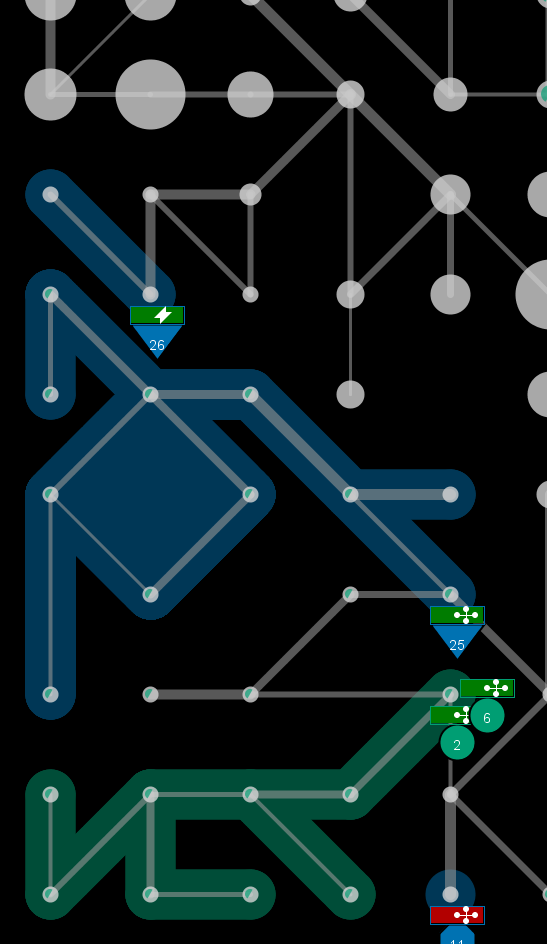
\includegraphics[height=.5\textheight]{images/articulation_points}
  \caption{By occupying an articulation point, a single agent can ostensibly establish a a high-scoring zone---provided that there are no enemy agents inside the subgraph that is split off from the main graph.}
  \label{fig:articulation_points}
\end{figure}
To position themselves in an optimally-scoring way, agents \emph{could} run the same algorithm locally to calculate the agent placement that will lead to the highest total sum of zone scores in each step by trying every possible permutation.
However, the number of ways to place $n$ agents on $k$ vertices is $C \left (n+r-1,r-1\right )= \frac{\left(n+r-1 \right )!}{n!\left(r-1 \right )!}$, a number that increases rapidly with $n$ and $k$.
In particular, there are $C \left (28+600-1,600-1 \right ) =\num{3.7463887025070038e+48}$ ways to place 28 agents on 600 vertices, which were the numbers used in the 2014 competition---far too many to calculate in real-time.
Finding an algorithm that calculates high-scoring zones in a limited computation time is one of the major challenges of the MAPC competition.

Our team developed a heuristic algorithm for calculating zones that will be explained below.
The goal is to find for every vertex in the graph a placement of agents around that vertex such that:
\begin{itemize}
  \item All vertices that share an edge with the centre vertex will be included in the zone.
  \item Agents should only be placed on the centre vertex's two-hop neighbours, which are those vertices that are be connected to the centre vertex through a minimum and maximum of two edges.
  \item The constructed zone's value per agent, that is, the sum of the values of each vertex in the zone divided by the numbers of agents required to establish that zone, should be high.
        Ideally, it would be maximal, but the heuristic we use doesn't guarantee this.
\end{itemize}
\autoref{fig:zones} shows some examples of zones that are found using our heuristic algorithm.
\begin{figure}
  \centering
  \subcaptionbox{This zone was calculated for a centre vertex that only has a degree of 1, i.e.\ that is a leaf vertex.
                 Generally, it is preferable to place an agent on the cut vertex that leads to a leaf vertex rather than the leaf vertex itself, as this would establish at least a zone of equal size, and possibly larger.
                 \label{fig:zones_1}}[.49\linewidth]{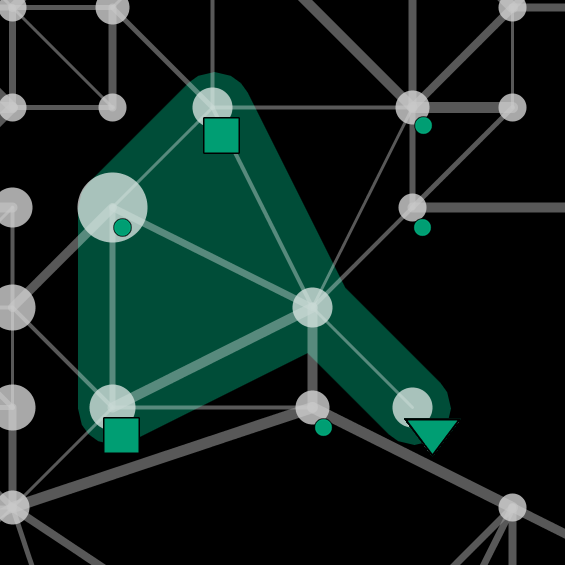
\includegraphics[width=.49\linewidth]{images/zone1.png}}
  \subcaptionbox{Here, the centre vertex has a degree of 3, and the calculated zone remains compact with only two additional agents used.
                 A lot of optional agent positions remain.
                 \label{fig:zones_2}}[.49\linewidth]{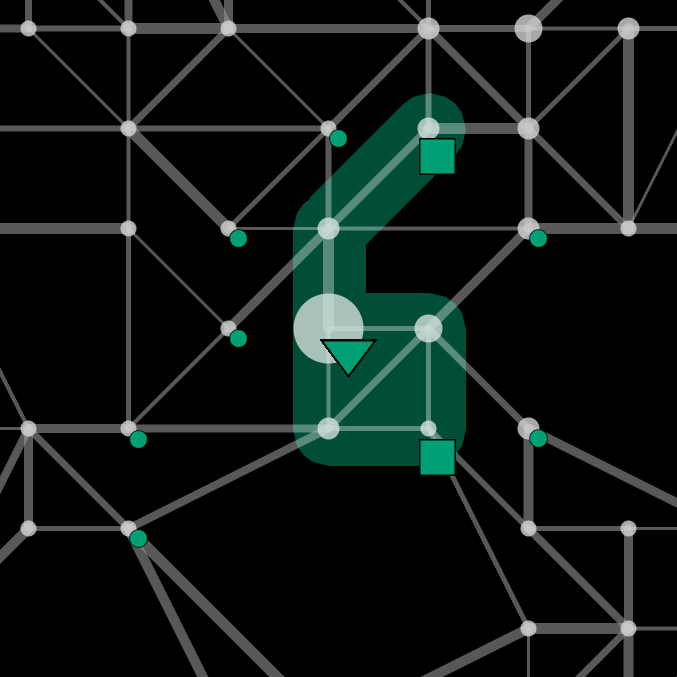
\includegraphics[width=.49\linewidth]{images/zone2.png}}
  \\
  \subcaptionbox{A zone where the centre vertex has a degree of 5, and the zone uses a total of 4 agents.
                 \label{fig:zones_3}}[.49\linewidth]{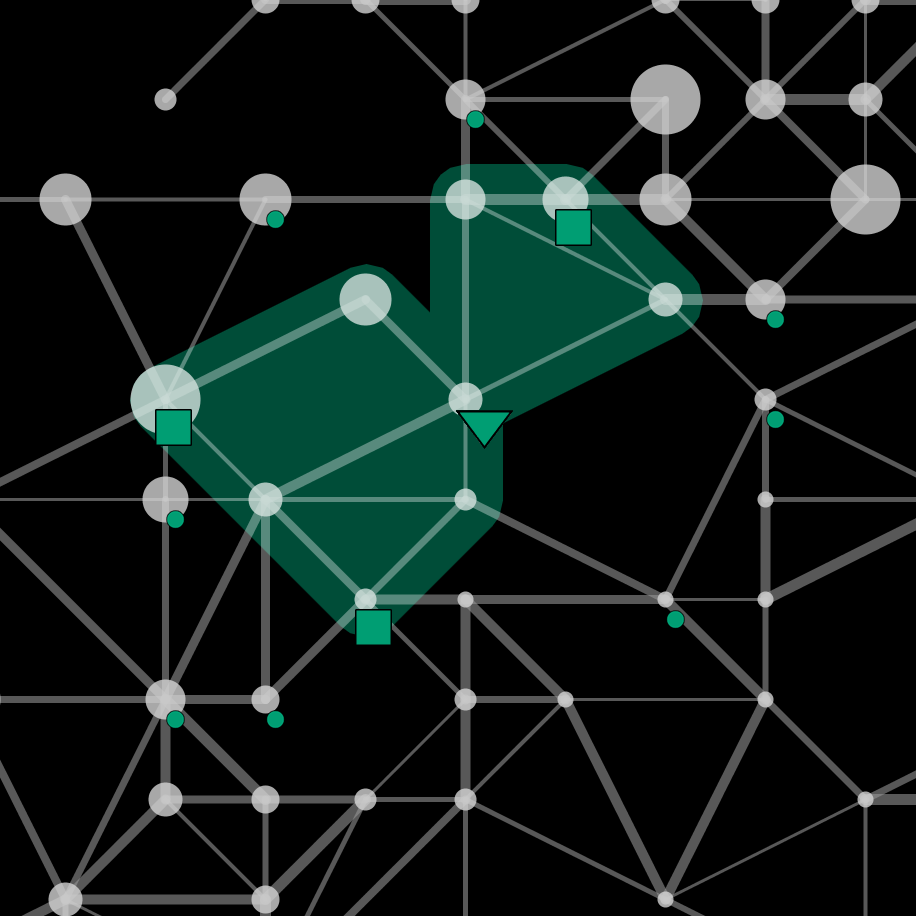
\includegraphics[width=.49\linewidth]{images/zone3.png}}
  \subcaptionbox{A zone where the centre vertex has a degree of 7, and the zone uses a total of 9 agents.
                 \label{fig:zones_4}}[.49\linewidth]{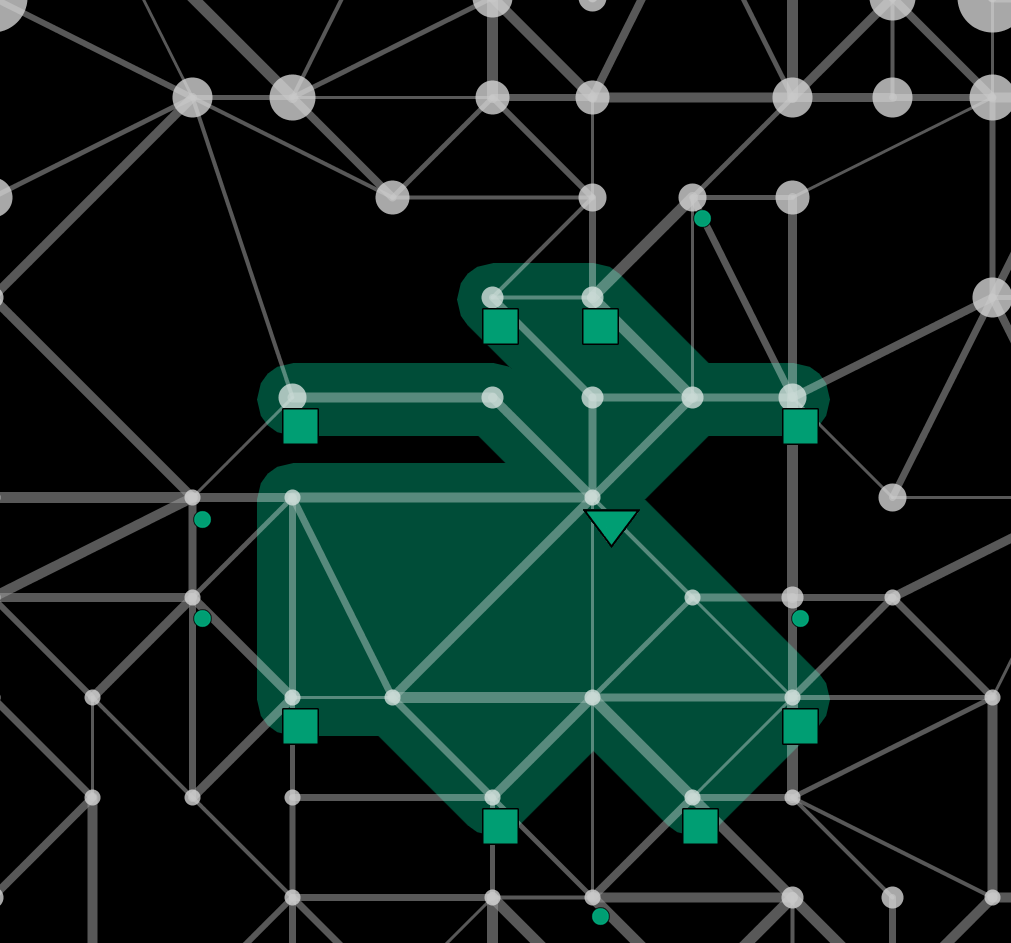
\includegraphics[width=.49\linewidth]{images/zone4.png}}
  \caption{Four examples of zones calculated by the heuristic algorithm described in \autoref{alg:zon_calculation}.
           The green squares and triangles represent the placement of agents, where the triangle is the agent on the center vertex.
           Vertices marked with a small green circle are optional agent positions that can be used to expand the zone if there are agents left over at the end of the zone building, as described in \autoref{alg:zon_finding}.
           The green-colored area represents the zone that is established by the given agent placement.}
  \label{fig:zones}
\end{figure}
Internally, every vertex in the graph is represented by a Java \lstinline{Vertex} object, and the calculated zone is stored as a field of that object.
The steps of the algorithm are best detailed graphically, as in \autoref{fig:coloring}.
\begin{definition}
  Let $V$ be the set of vertices and $E$ the set of edges that the system knows about.
  For any $v \in V$, which we will use to denote the vertex that a zone is centered on, let $V_v^1 \subseteq V$ be the set of one-hop neighbours of $v$, that is, the set of vertices that share an edge with $v$: $V_v^1= \left\{w \middle|\left(v,w \right ) \in E\right\}$.
  Similarly, $V_v^2$ denotes the set of two-hop neighbours of $v$, i.e.\ the set of vertices that includes exactly those vertices that share an edge with any vertex in $V_v^1$, excluding those in $V_v^1$ and $v$ itself: $V_v^2= \left\{u \middle|\left(v,w \right ) \in E, \left(w,u \right ) \in E, u \notin V_v^1\cup\{v\}\right\}$.
  Let $V_v^{2+}$ denote the entire two-hop neighbourhood of $v$: $V_{v}^{2+} = \{v\} \cup V_v^1 \cup V_v^2$.
  Additionally, let $A_v$ be an initially empty set that we will use to remember vertices we want to place agents on.
  A zone and its zone value are defined as specified by the graph colouring algorithm in~\cite{ahlbrecht_mapc_2014}.
  Then, the goal of the zone calculation algorithm is to find, for every $v \in V$ in the graph, a set of agent positions $A_v \subseteq V_{v}^{2+}$ that establish a zone around $v$ so that the zone's value \emph{per agent} is high according to the heuristic used by the algorithm.
\end{definition}
Note that although $V_v^1$ and $V_v^2$ start off as defined above, by abuse of notation we will remove vertices from those sets as the algorithm progresses.
This does not mean that the structure of the graph has changed.
The algorithm for zone calculation is (re)-triggered every time a vertex in the vertex' two-hop neighbourhood (so within the ambit of the zone we're trying to calculate) is discovered during map exploration or changes its known value when it is probed by an Explorer agent, as these are the events that can lead to possible changes in $A_v$ and thus the zone.

The zone centered around vertex $v$ is is calculated through several steps:
\begin{enumerate}
  \item Initially, $A_v = \emptyset$, and $V_v^1$, $V_v^2$ and $V_v^{2+}$ as defined above.
        Iterate through every $w \in V_v^2$ and, for every $w$ that is connected to 2 or more vertices in $V_v^1$, add it to $A_v$ and remove it from $V_v^2$:
        \begin{multline}
        \forall w \in V_v^2: \left\{\left(w, u_1 \right ), \left(w, u_2 \right )\right\} \subseteq E, u_1 \neq u_2, \left\{u_1, u_2\right\} \subseteq V_v^1 \\
        \rightarrow A_v := A_v \cup \left\{w\right\}, V_v^2 := V_v^2 \setminus \left\{w \right \}
        \end{multline}
  \item For every $w \in V_v^2$, if $w$ is connected either directly or through a single one-hop neighbour of $v$ to any $u \in A_v$, remove it from $V_v^2$: 
  \begin{multline}
  \forall w \in V_v^2: \exists u \in A_v: \rightarrow V_v^2 := V_v^2 \setminus \{w\}
\\ \forall w \in V_v^2: \exists u \in A_v: \exists x \in V_v^1: \left\{\left(w, x \right ), \left(x, u \right )\right\} \subseteq E\rightarrow V_v^2 := V_v^2 \setminus \{w\}
  \end{multline}
      The reasoning behind this is that those vertices in $V_v^1$ that are neighbours of those in $A_v$ will already definitely be included in the zone, and the vertices we remove this way will not contribute towards our goal of including all one-hop neighbours $V_v^1$ in the zone for $v$.
  \item In the next step, \enquote{bridges} are discovered in the list of remaining two-hop neighbours $V_v^2$.
        A \emph{bridge} is considered to be a connected triple of vertices where one of the vertices is directly connected to the other two.
        If such a bridge exists in $V_v^2$, all three involved vertices can be included in the zone around $v$ by placing an agent on either end of the of the bridge and leaving out the in-between vertex:
        \begin{multline}
        \forall w_1, w_2, w_3 \in V_v^2: \left(w_1, w_2\right ), \left(w_2, w_3 \right ) \in E \\ \rightarrow A_v := A_v \cup \left\{w_1, w_3 \right \}, V_v^2 := V_v^2 \setminus \left\{w_1,w_2,w_3\right\}
        \end{multline}
        Since three vertices can be captured in the zone for the \enquote{cost} of two agents, we consider this a good exchange to make.
  \item Next, the algorithm checks if all one-hop neighbours $V_v^1$ are connected to the agent positions $A_v$.
        This is frequently the case, but not always.
        If a remaining, unconnected one-hop $u \in V_v^1$ is found, we check if it is connected to one or more of the remaining two-hop vertices in $V_v^2$.
        If that is the case, we choose the neighbouring two-hop $w \in V_v^2$ with the highest vertex value and add it to the list of agent positions $A_v$.
        If no such two-hop vertex is found, we add the unconnected one-hop vertex to the list of agent positions---this is the only case where a one-hop vertex can be added to the list of agent positions: \begin{multline}
        \forall w \in V_v^1: \lnot \exists u \in A_v: \left(w, u \right ) \in E \\\rightarrow \left\{\begin{array}{lcl}
A_v := A_v \cup \left\{x\right\}, V_v^2 := V_v^2 \setminus \left\{x\right\} & \textup{if} & \exists x \in V_v^2: \left(x, w \right ) \in E\\
A_v := A_v \cup \left\{w\right\} &\textup{else} &
\end{array}\right.
        \end{multline}
  \item Finally, we include the center vertex $v$ in the list of agent positions: $A_v := A_v \cup \left\{v\right\}$.
        Any vertices that remain in $V_v^2$ are saved as additional agent positions that could be used to extend the zone by otherwise idle agents, but unlike the vertices in $A_v$ vertices are not required to establish the initial smallest zone that we calculated.
\end{enumerate}
\begin{figure}
  \centering
  \subcaptionbox{Before zone calculation.
                 \label{fig:coloring1}}[.49\linewidth]{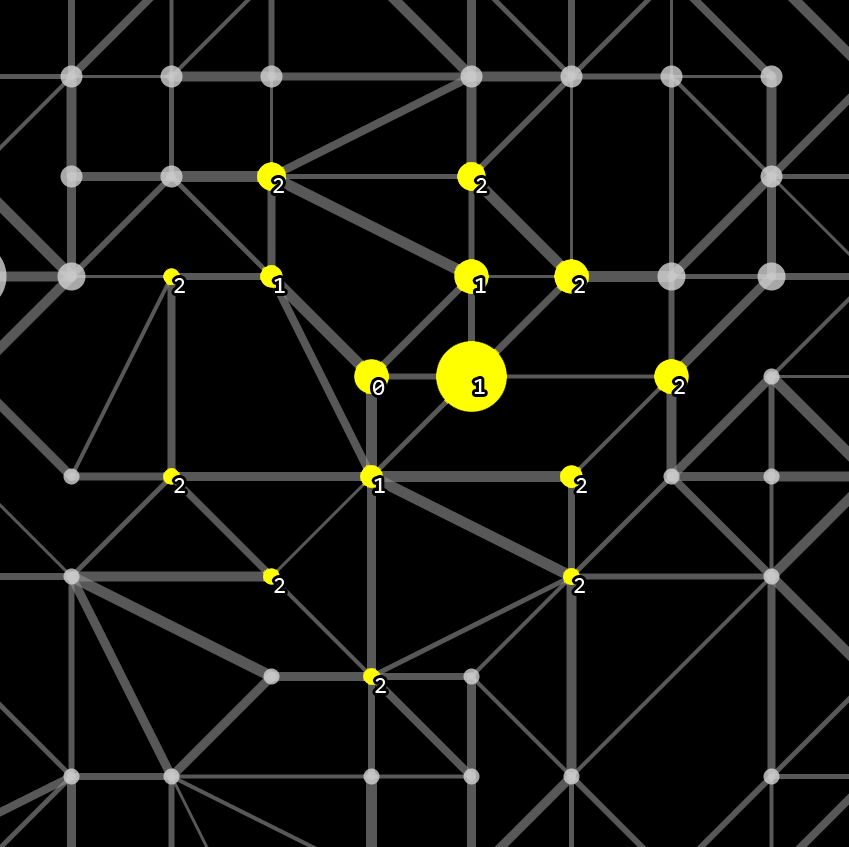
\includegraphics[width=.49\linewidth]{images/coloring1.png}}
  \subcaptionbox{After finding multiply-connected vertices in $V_v^2$ and removing their neighbouring two-hops.
                 \label{fig:coloring2}}[.49\linewidth]{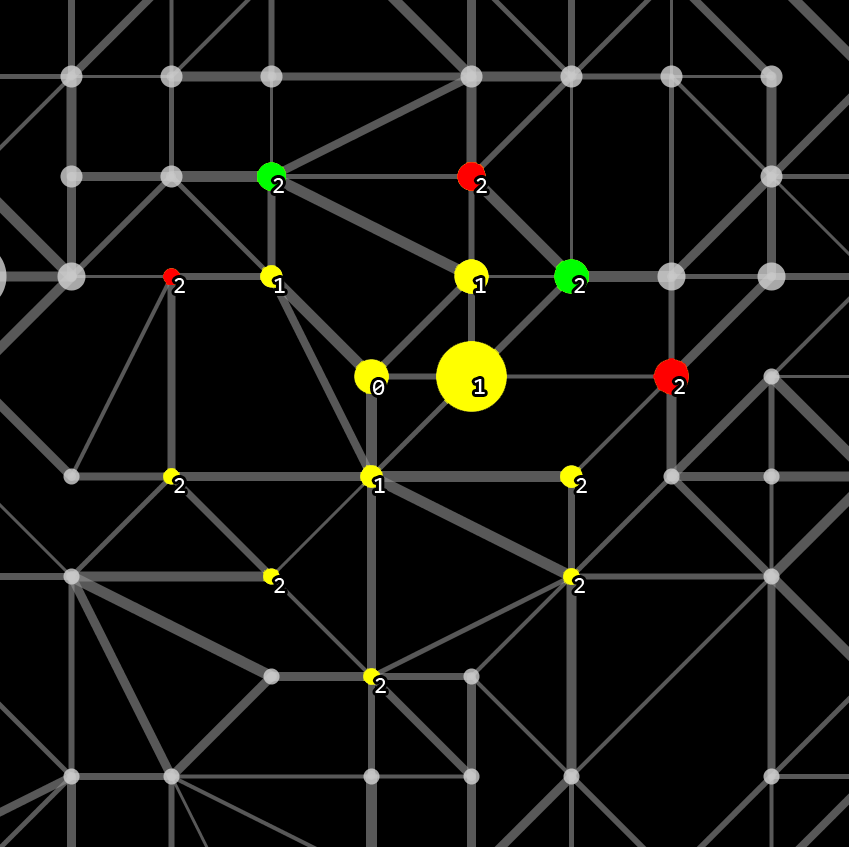
\includegraphics[width=.49\linewidth]{images/coloring2.png}}
  \\
  \subcaptionbox{Finding bridges.
                 \label{fig:coloring3}}[.49\linewidth]{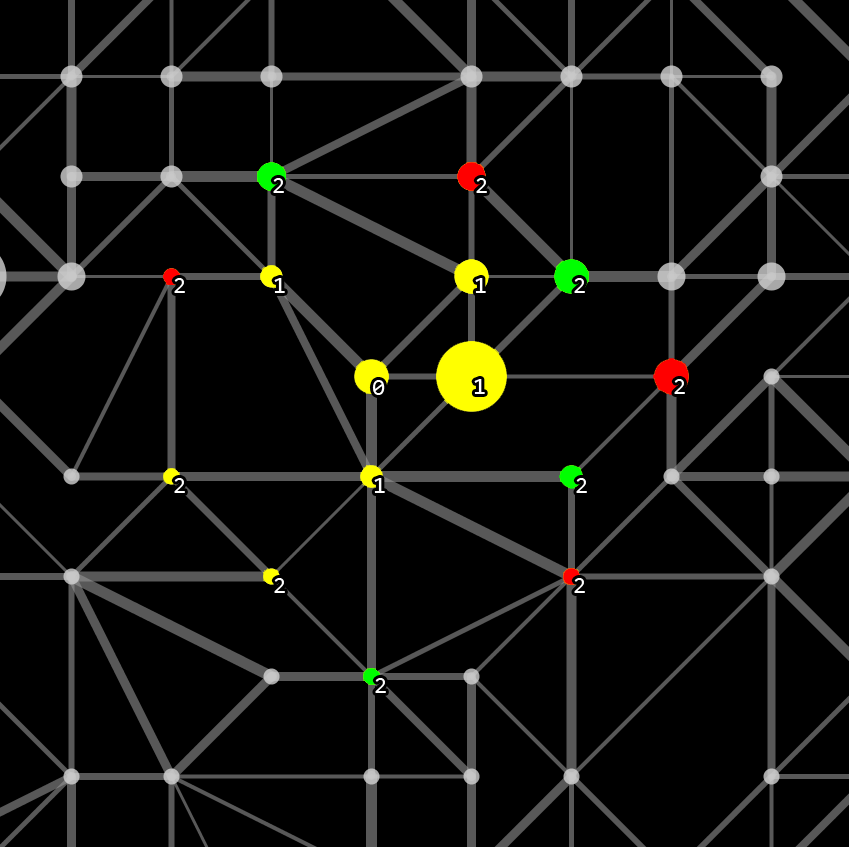
\includegraphics[width=.49\linewidth]{images/coloring3.png}}
  \subcaptionbox{After zone calculation.
                 \label{fig:coloring4}}[.49\linewidth]{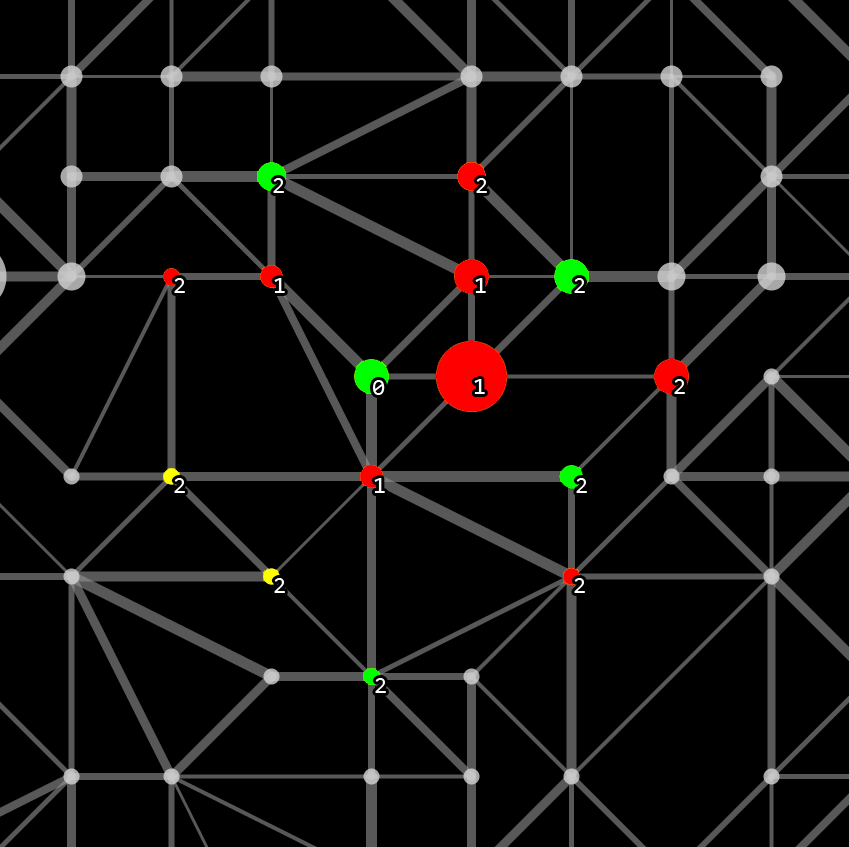
\includegraphics[width=.49\linewidth]{images/coloring4.png}}
  \caption{The zone calculation algorithm shown in four steps.
           Vertices are coloured differently according to their current state as the algorithm progresses.
           Green vertices are vertices that an agent must be placed on, so those in $A_v$.
           Red vertices are those where placing an agent would be redundant because it does not help with the goal of including all one-hop neighbours $V_v^1$ in the zone.
           Yellow vertices denote notes where agents could be placed to extend the zone, but are not considered optimal agent positions in the eyes of the algorithm.
           Numbers shown next to vertices represent their edge distance from the centre vertex $v$.}
  \label{fig:coloring}
\end{figure}
While we consider our algorithm to find zones of acceptably high zone values per agent, it can easily be shown to be suboptimal.
For one, it only considers vertices within the two-hop neighbourhood of the centre vertex, and it is not difficult to think of possible graph structures where a different agent placement would lead to a better zone.
For example, if one of the remaining yellow vertices in \autoref{fig:coloring4} were an articulation point whose inclusion in the list of agent positions would add more than that single vertex to the zone, this would probably be a good vertex to place an agent on, yet this would not be discovered by our heuristic algorithm.
